\section*{Теоретические вопросы}

\subsection*{1. Базис языка {\texttt{Lisp}}}

Базис -- это минимальный набор инструментов языка и стркутур данных, который позволяет решить любые задачи.

Базис Lisp :

\begin{itemize}
	\item[$-$] атомы и структуры (представляющиеся бинарными узлами);
	\item[$-$] базовые (несколько) функций и функционалов: встроенные — примитивные 
	функции (atom, eq, cons, car, cdr); специальные функции и функционалы (quote, 
	cond, lambda, eval, apply, funcall).
\end{itemize}
	
Функцией называется правило, по которому каждому значению одного или нескольких  аргументов ставится в соответствие конкретное значение результата.

Функционалом, или функцией высшего порядка называется функция, аргументом или  результатом которой является другая функция.

\subsection*{2. Классификация функций языка {\texttt{Lisp}}}

Функции в языке {\texttt{Lisp}}:
\begin{itemize}
	\item Чистые математические функции (имеют фиксированное количество аргументов, сначала выяисляются все аргументы, а только потом к ним применяется функция);
	\item Рекурсивные функции (основной способ выполнения повторных вычислений);
	\item Специальные функции, или формы (могут принимать произвольное количество аргументов, или аргументы могут обрабатываться по-разному);
	\item Псевдофункции (создают «эффект», например, вывод на экран);
	\item Функции с вариантами значений, из которых выбирается одно;
	\item Функции высших порядков, или функционалы --  функции, аргументом или  результатом которых является другая функция (используются для построения синтаксически управляемых программ)
	\item Базисные функции --- минимальный набор функций, позволяющих решить любую задачу.
\end{itemize}

Также базисные и функции ядра можно классифицировать с точки \\зрения действий.
\begin{enumerate}
	\item Селекторы --- переходят по соответствующему указателю списковой ячейки.
	\item Конструкторы --- создают структуры данных.
	\item Предикаты --- позволяют классифицировать или сравнивать структуры.
\end{enumerate}

\subsection*{3. Способы создания функций}

\begin{itemize}
	\item С помощью lambda. После ключевого слова указывается лямбда-список и тело функции. 
	\begin{lstlisting}
(lambda (x y) (+ x y))
	\end{lstlisting}
	Для применения используются лямбда-выражения.
	\begin{lstlisting}
((lambda (x y) (+ x y)) 1 2)
	\end{lstlisting}
	\item С помощью defun. Используется для неоднократного применения функции (в том числе рекурсивного вызова).
	\begin{lstlisting}
(defun sum (x y) (+ x y))
(sum 1 2)
	\end{lstlisting}

\end{itemize}

\subsection*{4. Функции Car и Cdr, eq, eql, equal, equalp}

\begin{itemize}
	\item Функция car от одного аргумента возвращает первый элемент списка, являющегося значением её аргумента;
	\item Функция cdr возвращает хвост списка, являющегося значением её единственного аргумента (хвостом, или остатком списка является список  без своего первого элемента);
	\item Функция eq корректно сравнивает два символьных атома. Так как атомы не дублирутюся для данного сеанса работы, то фактически сравниваются соответсвующие указатели;
	Возвращает T, когда: 
		\begin{enumerate}
			\item значением одного из аргументов является атом, и одновременно;
			\item значения аргументов равны (идентичны). В ином случае значением функции eq является NIL. (eq  'ab 'Ab) => T, но (eq 1 2) => NIL.
		\end{enumerate}
	\item Функция eql корректно сравнивает атомы и числа одинакового типа (синтетической формы записи). Например, (eql 1 1) вернет T, а (eql 1 1.0) -- Nil, так как целое значение 1 и значение с плавающей точкой 1.0 являются представителями различных классов;
	\item Функция equal работает идентично eql, но в дополнение умеет корректно сравнивать списки (считая списки эквивалентными, если они рекурсивно, согласно тому же equal, имеют одинаковую структуру и содержимое; считая строки эквивалентными, если они содержат одинаковые знаки);
	\item Функция equalp корректно сравнивает любые S-выражения. 
\end{itemize}

\subsection*{5. Назначение и отличие в работе Cons и List}

Cons --- функция от двух аргументов. Создает списковую ячейку и расставляет 2 указателя -- на голову и на хвост -- на входные аргументы.

List --- функция от произвольного числа аргументов, при этом все они вычисляются. Строит новый список, первым элементом которого является значение первого аргумента, хвостом -- значение второго аргумента.

\begin{lstlisting}
(cons '(A) '(B)) ;; ((A) B)
(list '(A) '(B)) ;; ((A) (B))
\end{lstlisting}

\newpage
\section*{Практические задания}
\subsection*{1. Задание 1}
Составить диаграмму вычисления следующих выражений:

\begin{enumerate}
	\item (equal 3 (abs -3))

	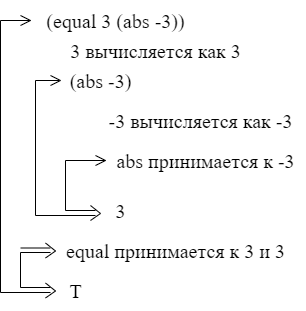
\includegraphics[scale=1.0]{img/1.1}	

	\item (equal (+ 1 2) 3)	

	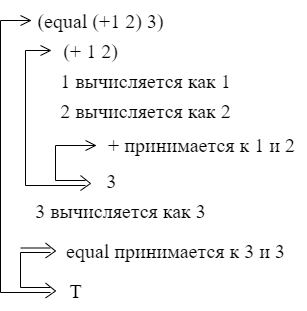
\includegraphics[scale=1.0]{img/1.2}	
\newpage
	\item (equal (* 4 7) 21)

	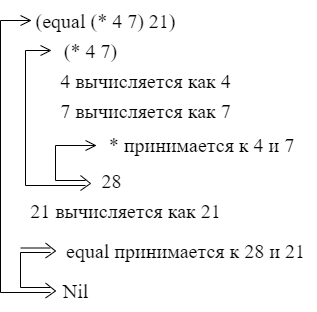
\includegraphics[scale=1.0]{img/1.3}	

	\item (equal (* 2 3) (+ 7 2))

	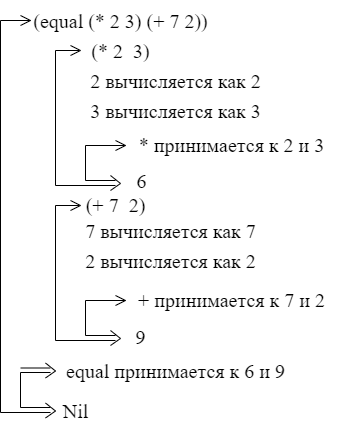
\includegraphics[scale=1.0]{img/1.4}	

	\item (equal (- 7 3) (* 3 2))
\newpage
	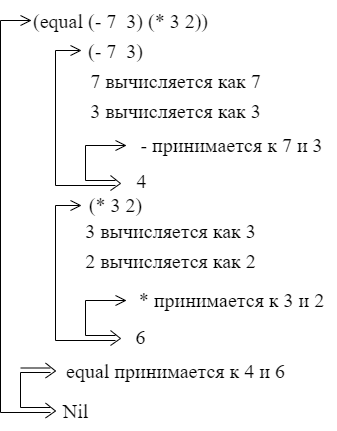
\includegraphics[scale=1.0]{img/1.5}	

	\item (equal (abs (- 2 4)) 3))

	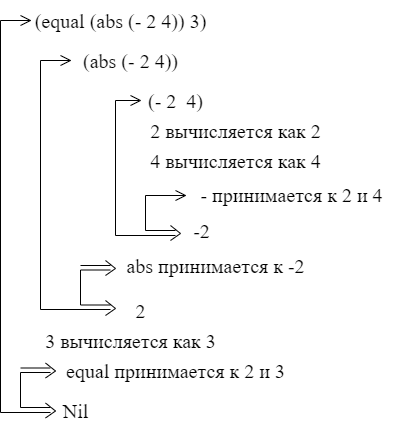
\includegraphics[scale=1.0]{img/1.6}	
\end{enumerate}
\newpage
\subsection*{2. Задание 2}
Написать функцию, вычисляющую гипотенузу прямоугольного
треугольника по заданным катетам и составить диаграмму её вычисления.

\begin{lstlisting}
(defun hypotenuse (a b) (sqrt (+ (* a a) (* b b))))
(hypotenuse 3 4)  => 5.0
\end{lstlisting}

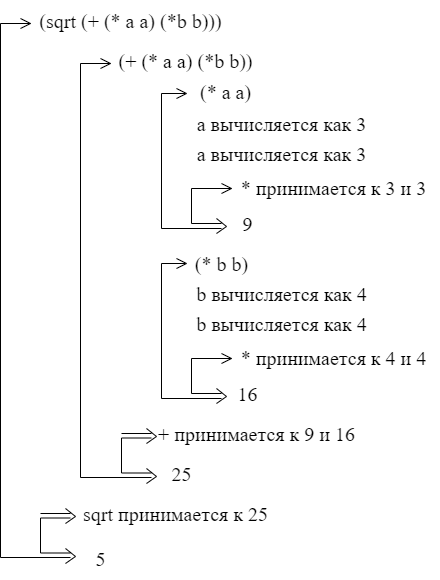
\includegraphics[scale=1.0]{img/2}	
\newpage
\subsection*{3. Задание 3}
Каковы результаты вычисления следующих выражений?(объяснить возможную ошибку и варианты ее устранен6ия)

\begin{lstlisting}
(list 'a c) ; The variable C is unbound.
=> (list 'a 'c) 

(cons 'a (b c)) ; Undefined function : B, Undefined variable : C
=> (cons 'a '(b c))

(cons 'a '(b c)) => (A B C)

(caddr (1 2 3 4 5)) ;illegal function call
=> (caddr '(1 2 3 4 5))

(cons 'a 'b 'c) 
;The function CONS is called with three arguments, but wants exactly two.
=> (list 'a 'b 'c)

(list 'a (b c)) ; Undefined function : B, Undefined variable : C
=> (list 'a '(b c))

(list a '(b c)) ; The variable A is unbound.
=> (list 'a '(b c))

(list (+ 1 '(length '(1 2 3)))) 
;The value (LENGTH '(1 2 3)) is not of type NUMBER
=> (list (+ 1 (length '(1 2 3))))
\end{lstlisting}

\subsection*{4. Задание 4}
Написать функцию longer\_then от двух списков-аргументов, которая возвращает Т, если первый аргумент имеет большую длину.
\begin{lstlisting}
(defun longer_then (list1 list2) (> (length list 1) (length list2)))
\end{lstlisting}

\subsection*{5. Задание 5}
Каковы результаты вычисления следующих выражений?
\begin{lstlisting}
(cons 3 (list 5 6)) =>	(3 5 6)
(cons 3 '(list 5 6)) => (3 LIST 5 6)
(list 3 'from 9 'lives (- 9 3))	 => (3 FROM 9 LIVES 6)
(+ (length for 2 too)) (car '(21 22 23))) ;The variable FOR is unbound.
(cdr '(cons is short for ans)) => (IS SHORT FOR ANS)
(car (list one two))	 ;The variable ONE is unbound.
(car (list 'one 'two)) => ONE
\end{lstlisting}

\subsection*{6. Задание 6}
Дана функция (defun mystery (x) (list (second x) (first x))). Какие результаты вычисления следующих выражений?

\begin{lstlisting}
(mystery (one two)) ;The variable TWO is unbound.
(mystery (last one two)) ;The variable ONE is unbound.
(mystery free) ;The variable FREE is unbound.
(mystery one 'two)) ;The variable ONE is unbound.
\end{lstlisting}

\subsection*{7. Задание 7}
Написать функцию, которая переводит температуру в системе Фаренгейта
температуру по Цельсию (defum f-to-c (temp)…).
\begin{lstlisting}
(defun f_to_c (temp) (* (/ 5 9) (- temp 32.0)))
(f_to_c 451) => 232.77779
\end{lstlisting}

\subsection*{8. Задание 8}
Что получится при вычисления каждого из выражений?
\begin{lstlisting}
(list 'cons t NIL) => (CONS T NIL)
(eval (eval (list 'cons t NIL))) ;The function COMMON-LISP:T is undefined
(apply 'cons '(t NIL)) => (T)
(list 'eval NIL) => (EVAL NIL)
(eval (list 'cons t NIL))  => (T)
(eval NIL) => NIL
(eval (list 'eval NIL)) => NIL
\end{lstlisting}

